\documentclass{article}
\usepackage{tikz}
\usepackage{geometry}
\usepackage{float}
\usepackage{caption}
\usetikzlibrary{automata,positioning,backgrounds,calc,arrows.meta,shapes.geometric,fit,shadows}

% Setting page geometry for better display
\geometry{a4paper, landscape, margin=0.5in}

\begin{document}

\begin{figure}[H]
    \centering
    % Resizing to fit the landscape page width
    \resizebox{1.0\textwidth}{!}{%
    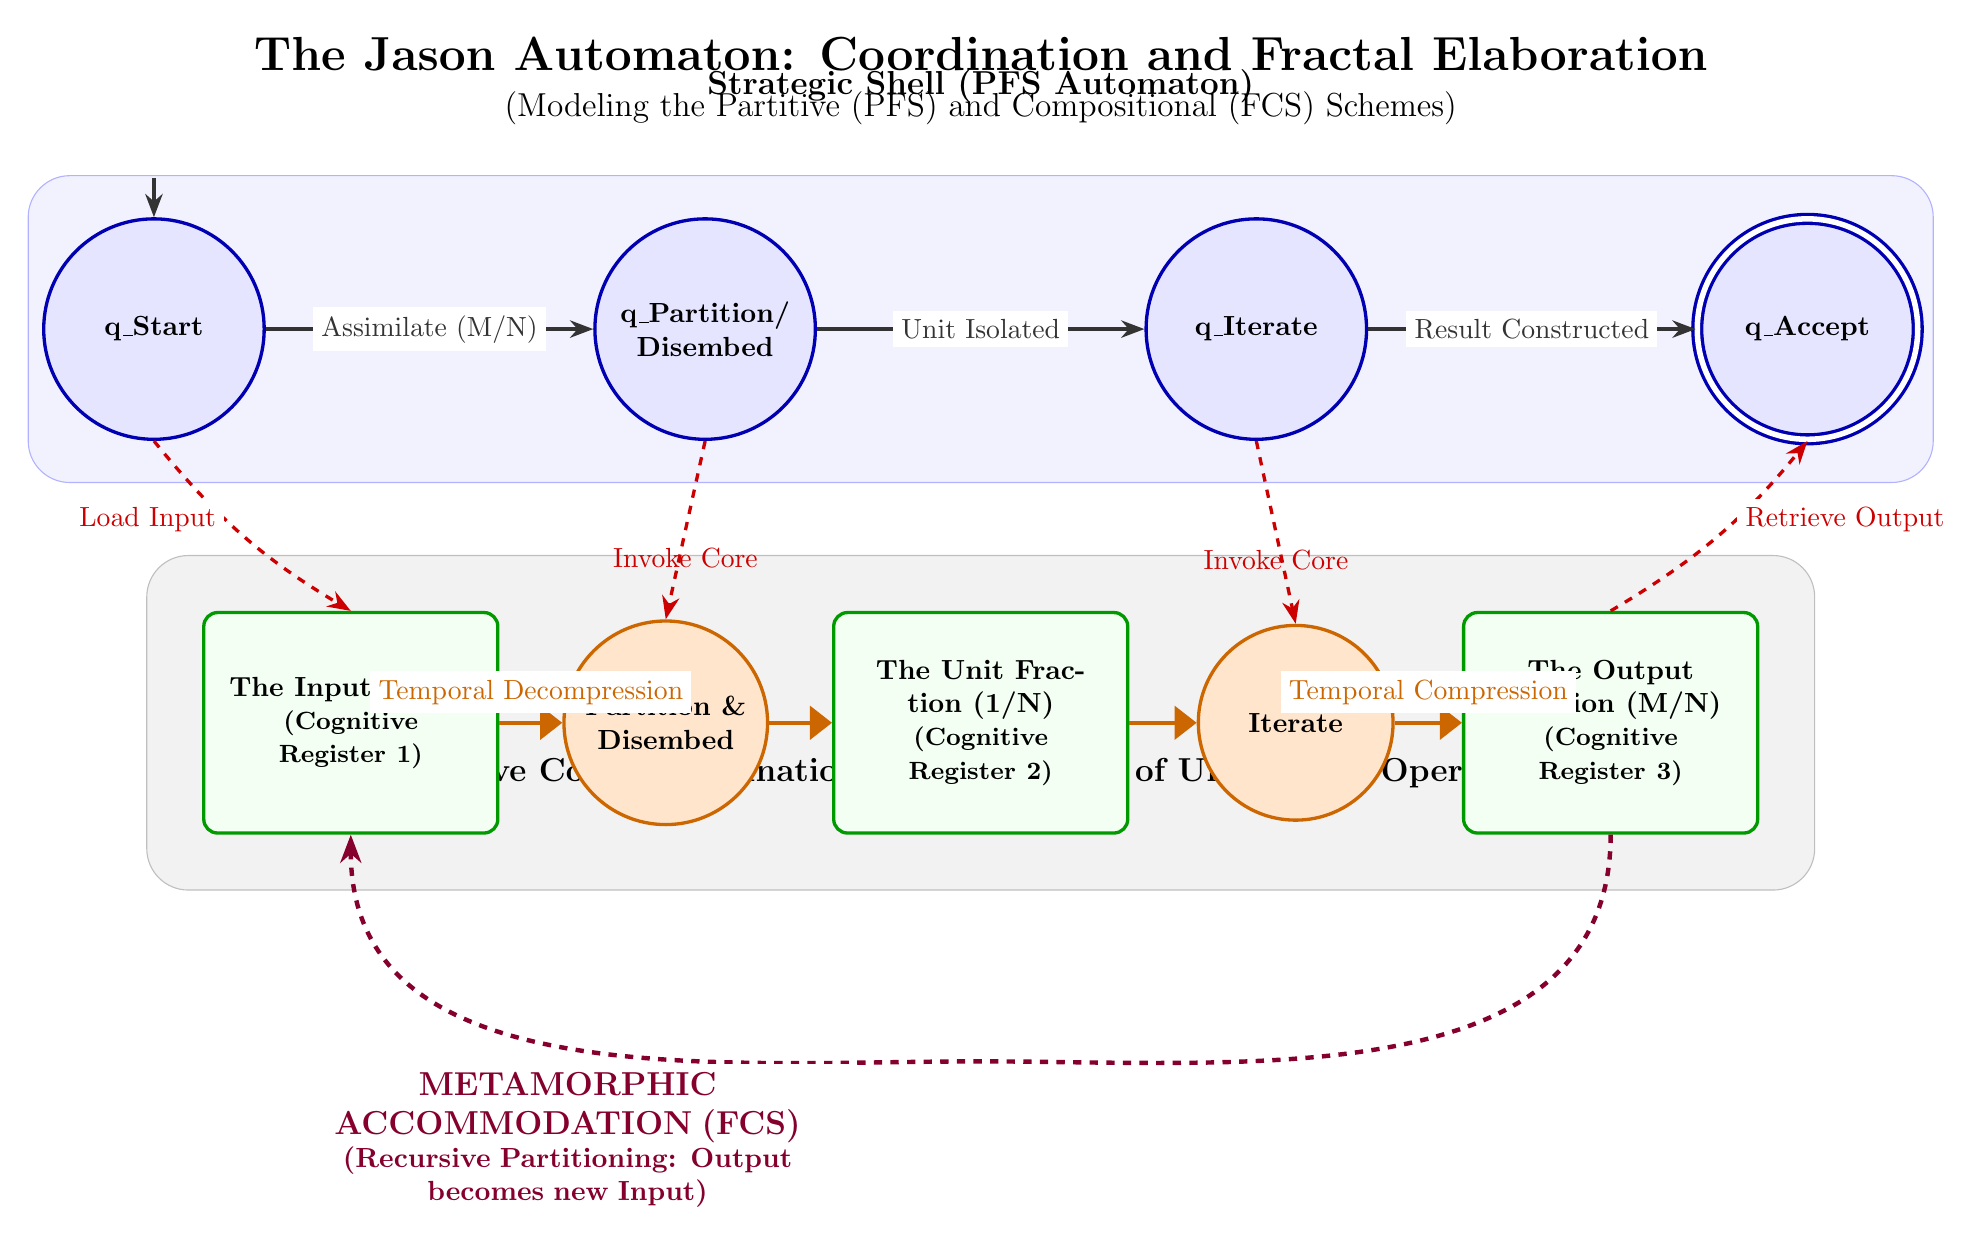
\begin{tikzpicture}[
        node distance=3cm,
        >=Stealth,
        shell_state/.style={
            circle, 
            draw=blue!70!black, 
            fill=blue!10, 
            very thick, 
            minimum size=2.8cm, 
            text width=2.4cm, 
            align=center, 
            font=\bfseries
        },
        unit_level/.style={
            rectangle, 
            draw=green!60!black, 
            fill=green!5, 
            very thick, 
            minimum height=2.8cm, 
            text width=3.5cm, 
            align=center, 
            font=\bfseries,
            rounded corners=5pt
        },
        core_op/.style={
            circle, 
            draw=orange!80!black, 
            fill=orange!20, 
            very thick,
            minimum size=2cm, 
            text width=2.2cm, 
            align=center, 
            font=\bfseries
        },
        accepting_style/.style={double, double distance=2pt},
        shell_arrow/.style={-Stealth, very thick, black!80},
        core_arrow/.style={-{Triangle[width=12pt,length=8pt]}, ultra thick, orange!80!black},
        invocation_arrow/.style={-Stealth, very thick, red!80!black, dashed},
        recursion_arrow/.style={-Stealth, ultra thick, purple!70!black, dashed},
        title/.style={font=\bfseries\LARGE},
        subtitle/.style={font=\large},
        label_text/.style={font=\normalsize, fill=white, inner sep=3pt, midway, align=center}
    ]

    % Title
    \node[title] at (0, 11) {The Jason Automaton: Coordination and Fractal Elaboration};
    \node[subtitle] at (0, 10.3) {(Modeling the Partitive (PFS) and Compositional (FCS) Schemes)};

    % =================================================
    % THE ITERATIVE CORE (Coordination Mechanism)
    % =================================================
    
    % Unit Levels (The three coordinated quantities / registers)
    \node[unit_level] (L1_Whole) at (-8, 2.5) {The Input Whole \\ \small(Cognitive Register 1)};
    \node[unit_level] (L2_UnitFrac) at (0, 2.5) {The Unit Fraction (1/N) \\ \small(Cognitive Register 2)};
    \node[unit_level] (L3_ResultFrac) at (8, 2.5) {The Output Fraction (M/N) \\ \small(Cognitive Register 3)};

    % Core Operations (The "Gears" mediating transformations)
    \node[core_op] (Op_PartDis) at (-4, 2.5) {Partition \& Disembed};
    \node[core_op] (Op_Iterate) at (4, 2.5) {Iterate};

    % Core Arrows (Data Flow / Transformation)
    \draw[core_arrow] (L1_Whole.east) -- node[label_text, above, yshift=0.1cm] {Temporal Decompression} (Op_PartDis.west);
    \draw[core_arrow] (Op_PartDis.east) -- (L2_UnitFrac.west);
    \draw[core_arrow] (L2_UnitFrac.east) -- (Op_Iterate.west);
    \draw[core_arrow] (Op_Iterate.east) -- node[label_text, above, yshift=0.1cm] {Temporal Compression} (L3_ResultFrac.west);

    % Background for the Core
    \begin{pgfonlayer}{background}
        \node[fit={(L1_Whole) (L3_ResultFrac) (Op_PartDis)}, draw=gray!50, fill=gray!10, rounded corners=15pt, inner sep=20pt, label={[yshift=-3.1cm, font=\large\bfseries]{Iterative Core: Coordination of Three Levels of Units (ENS Operations)}}] (CoreBox) {};
    \end{pgfonlayer}

    % =================================================
    % THE STRATEGIC SHELL (PFS Automaton)
    % =================================================

    % Shell States (Control Flow)
    \node[shell_state] (q_Start) at (-10.5, 7.5) {q\_Start};
    \node[shell_state] (q_Part) at (-3.5, 7.5) {q\_Partition/\\Disembed};
    \node[shell_state] (q_Iterate) at (3.5, 7.5) {q\_Iterate};
    \node[shell_state, accepting_style] (q_Accept) at (10.5, 7.5) {q\_Accept};

    % Shell Transitions (The Choreography)
    \draw[shell_arrow] (q_Start.east) -- node[label_text] {Assimilate (M/N)} (q_Part.west);
    \draw[shell_arrow] (q_Part.east) -- node[label_text] {Unit Isolated} (q_Iterate.west);
    \draw[shell_arrow] (q_Iterate.east) -- node[label_text] {Result Constructed} (q_Accept.west);

    % Start indicator
    \draw[shell_arrow] ([yshift=0.5cm]q_Start.north) -- (q_Start.north);
    
    % Background for the Shell
    \begin{pgfonlayer}{background}
        \node[fit={(q_Start) (q_Accept)}, draw=blue!30, fill=blue!5, rounded corners=15pt, inner ysep=15pt, inner xsep=5pt, label={[yshift=0.8cm, font=\large\bfseries]{Strategic Shell (PFS Automaton)}}] (ShellBox) {};
    \end{pgfonlayer}

    % =================================================
    % ORCHESTRATION (Shell Invoking Core)
    % =================================================

    \draw[invocation_arrow] (q_Start.south) to[bend right=10] node[label_text, pos=0.4, left] {Load Input} (L1_Whole.north);
    \draw[invocation_arrow] (q_Part.south) -- node[label_text, fill=none, below, yshift=-0.1cm] {Invoke Core} (Op_PartDis.north);
    \draw[invocation_arrow] (q_Iterate.south) -- node[label_text, fill=none, below, yshift=-0.1cm] {Invoke Core} (Op_Iterate.north);
    \draw[invocation_arrow] (L3_ResultFrac.north) to[bend right=10] node[label_text, pos=0.6, right] {Retrieve Output} (q_Accept.south);

    % =================================================
    % FRACTAL ELABORATION (FCS Recursion)
    % =================================================

    \draw[recursion_arrow] (L3_ResultFrac.south) to[out=-90, in=0] (0, -1.8) to[out=180, in=-90] 
    node[label_text, below, yshift=-0.2cm, text width=7cm]
    {\parbox{7cm}{\centering\large\bfseries\color{purple!70!black}METAMORPHIC ACCOMMODATION (FCS) \\ \normalsize(Recursive Partitioning: Output becomes new Input)}} 
    (L1_Whole.south);

    \end{tikzpicture}%
    }
    \caption{Visualization of Jason's fractional reasoning architecture. The Strategic Shell (PFS) choreographs the Iterative Core (ENS Operations) to coordinate the Three Levels of Units (Input Whole, Unit Fraction, Output Fraction). The recursive pathway (purple) illustrates the reorganization into the Fractional Composition Scheme (FCS), where the scheme operates on its own output (fractal elaboration).}
    \label{fig:jason-automata-coordination}
\end{figure}

\end{document}